\documentclass{article}
\usepackage{tikz}
\usetikzlibrary{automata,arrows}
\begin{document}
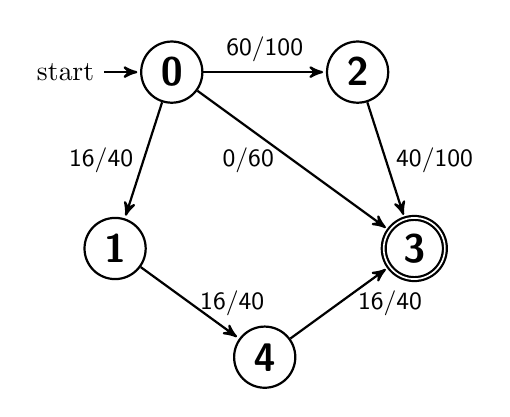
\begin{tikzpicture}[->,>=stealth',shorten >=1pt,auto,node distance=3cm,
                    thick,main node/.style={circle,draw,font=\sffamily\Large\bfseries}]

  \node[initial,main node] (0) at (9.82,12.62) {0};
  \node[main node] (1) at (9.1,10.38) {1};
  \node[main node] (2) at (12.18,12.62) {2};
  \node[main node,accepting] (3) at (12.9,10.38) {3};
  \node[main node] (4) at (11,9) {4};

  \path[every node/.style={font=\sffamily\small}]
    (0) edge node [above] {60/100} (2)
        edge [left] node[left] {16/40} (1)
        edge [left] node[left] {0/60\ \ } (3)
    (1) edge node [right] {16/40} (4)
    (2) edge [right] node[right] {40/100} (3)
    (4) edge node [right] {\ 16/40} (3);
\end{tikzpicture}
\end{document}
